%20 min preso!
\documentclass[xcolor=table]{beamer}
\usepackage{beamerthemesplit}
\usepackage{wrapfig}
\usetheme{SPbGU}
\usepackage{pdfpages}
\usepackage{amsmath}
\usepackage{cmap}
\usepackage[T2A]{fontenc}
\usepackage[utf8]{inputenc}
\usepackage[english]{babel}
\usepackage{indentfirst}
\usepackage{amsmath}
\usepackage{tikz}
\usepackage{multirow}
\usepackage[noend]{algpseudocode}
\usepackage{algorithm}
\usepackage{algorithmicx}
\usepackage{fancyvrb}
\usetikzlibrary{calc}
\usetikzlibrary{shapes,arrows}
\usetikzlibrary{arrows,automata}
\usetikzlibrary{positioning}

\usepackage{tabularx}
\newcolumntype{Y}{>{\raggedleft\arraybackslash}X}

\renewcommand{\thealgorithm}{}

\newtheorem{mytheorem}{Theorem}
\renewcommand{\thealgorithm}{}

\newcommand{\tikzmark}[1]{\tikz[overlay,remember picture] \node (#1) {};}
\def\Put(#1,#2)#3{\leavevmode\makebox(0,0){\put(#1,#2){#3}}}

\newcommand{\ltz}{$< 1$}


\tikzset{
    state/.style={
           rectangle,
           rounded corners,
           draw=black, very thick,
           minimum height=2em,
           inner sep=2pt,
           text centered,
           },
}

\beamertemplatenavigationsymbolsempty

\title[Single-Path CFPQ]{Context-Free Path Querying with Single-Path Semantics by Matrix Multiplication}
%\subtitle[YaccConstructor]{Parsing techniques for graph analysis}
% То, что в квадратных скобках, отображается в левом нижнем углу.
\institute[JetBrains Research]{
JetBrains Research, Programming Languages and Tools Lab  \\
Saint Petersburg University
}

% То, что в квадратных скобках, отображается в левом нижнем углу.
\author[Rustam Azimov]{Arseniy Terekhov, Artyom Khoroshev, \\ Semyon Grigorev, \textbf{Rustam Azimov}}

\date{June 14, 2020}

\begin{document}
{
\begin{frame}[fragile]
  \begin{table}
  \centering
  \begin{tabularx}{\linewidth}{YcX}
    
\includegraphics[height=1.5cm]{pictures/jetbrainsResearch.pdf} \hfill
    & \begin{minipage}[t]{0.3\textwidth}\center \vspace{-1cm}  GRADES-NDA 2020
      \end{minipage}
    & \hfill 
\includegraphics[height=1.5cm]{pictures/SPbGU_Logo.png}
  \end{tabularx}
  \end{table}
  \titlepage
\end{frame}
}

\begin{frame} \frametitle{Context-Free Path Querying}
  \begin{minipage}[m]{0.45\linewidth}
  \raisebox{-0.5\totalheight}{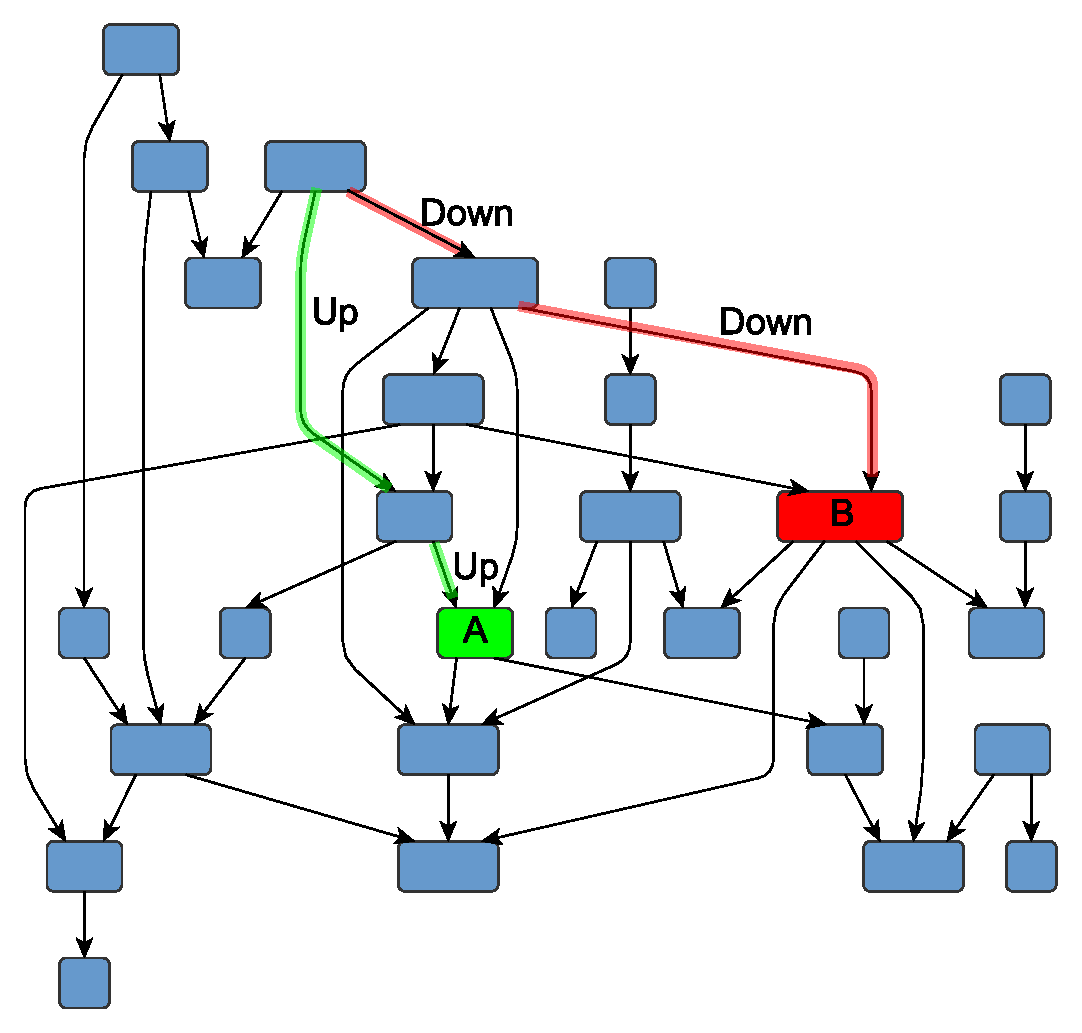
\includegraphics[width=\textwidth]{pictures/hierarchical.pdf}}
  \end{minipage}\hfill
  \begin{minipage}[m]{0.5\linewidth}
  Navigation through a graph
  \begin{itemize}
        \item Are nodes A and B on the same level of hierarchy?
        \item Is there a path of form $\textbf{Up}^n \, \textbf{Down}^n$?
        \item Find all paths of form $\textbf{Up}^n \, \textbf{Down}^n$ which start from the~node A
  \end{itemize}

  \end{minipage}

  \end{frame}

%  \begin{frame}[fragile] \frametitle{Applicatipons}
%    \begin{itemize}
%      \item Static code analysis
%      \item Graph database querying
%      \item RDF analysis
%    \end{itemize}
%  \end{frame}

  \begin{frame}[fragile]
    \frametitle{Context-Free Path Querying: Relational Query Semantics}
    \begin{itemize}
      \item $\mathbb{G} = (\Sigma, N, P)$ --- context-free grammar in normal form
      \begin{itemize}
        \item $A \rightarrow B C$, where $A, B, C \in N$
        \item $A \rightarrow x$, where $A \in N, x \in \Sigma \cup \{\varepsilon\}$
        \item $L(\mathbb{G},A) = \{ \omega \mid A \Rightarrow^* \omega \}$
      \end{itemize}
      \pause
      \item $G = (V,E,L)$ --- directed graph
        \begin{itemize}
          \item $v \xrightarrow{l} u \in E$
          \item $L \subseteq \Sigma$
        \end{itemize}
        \pause
      %\item $p = v_0 \xrightarrow{l_0} v_1 \xrightarrow{l_1} \cdots \xrightarrow{l_{n-2}} v_{n-1} \xrightarrow{l_{n-1}} v_n$ --- path in $G$
      \item $\omega(\pi) = \omega(v_0 \xrightarrow{l_0} v_1 \xrightarrow{l_1} \cdots \xrightarrow{l_{n-2}} v_{n-1} \xrightarrow{l_{n-1}} v_n) = l_0 l_1 \cdots l_{n-1}$
      \pause
      \item $R_A = \{ (n, m) \mid \exists n \pi m$, such that $\omega(\pi) \in L(\mathbb{G},A)\}$
    \end{itemize}
  \end{frame}

  \begin{frame}[fragile] \frametitle{Matrix-Based Algorithm: Relational Query Semantics}
    	\begin{algorithm}[H]
    		\begin{algorithmic}[1]
    			\caption{Context-free path querying algorithm}
    			\label{lst:algo1}
    			\Function{evalCFPQ}{$D=(V,E,L), G=(\Sigma,N,P)$}
    			\State{$n \gets$ |V|}
    			\State{$T \gets \{T^{A_i} \mid A_i \in N, T^{A_i}$ is a matrix $n \times n$, $T^{A_i}_{k,l} \gets$ \texttt{false}\} }
    			\ForAll{$(i,x,j) \in E$, $A_k \mid A_k \to x \in P$}
    			%\Comment{Matrices initialization}
    			%\For{$A_k \mid A_k \to x \in P$}
    			{$T^{A_k}_{i,j} \gets \texttt{true}$}
    			%\EndFor
    			\EndFor
    			\ForAll{$A_k \mid A_k \to \varepsilon \in P$}
    			\ForAll{$i \in \{0,\ldots ,n-1\}$}
    			{$T^{A_k}_{i,i} \gets \texttt{true}$}
    			\EndFor
    			\EndFor
    			
    			\While{any matrix in $T$ is changing}
    			%\Comment{Transitive c	losure calculation}
    			\For{$A_i \to A_j A_k \in P$}
    			{ $T^{A_i} \gets T^{A_i} + (T^{A_j} \times T^{A_k})$ } 
    			\EndFor
    			\EndWhile
    			\State \Return $T$
    			\EndFunction
    		\end{algorithmic}
    	\end{algorithm}
  \end{frame}


\begin{frame}[fragile]
\frametitle{Context-Free Path Querying: Single-Path Query Semantics}
\begin{itemize}
	\item $R_A = \{ (n, m) \mid \exists n \pi m$, such that $\omega(\pi) \in L(\mathbb{G},A)\}$ --- answers for the relational query semantics
	\pause
	\item For all $A \in N$, for all $(n,m) \in R_A$ also return some such path $n\pi m$
	\begin{itemize}
		\item usually the shortest path is returned
		\item returned path can be used as a proof of existence
	\end{itemize}
	
\end{itemize}
\end{frame}

\begin{frame}[fragile] \frametitle{Research Questions}
\begin{itemize}
	\item Can we extend the matrix-based CFPQ algorithm to single-path query semantics?
	\item What the cost of such extension?
	\item Can we achieve high performance of CFPQ integrated with existing graph database?
	\item Does using GPGPU still improve performance over CPU versions?
\end{itemize}
\end{frame}

\begin{frame}[fragile] \frametitle{Path Index}
\begin{itemize}
	\item $\textit{PathIndex} = (\textit{left},\textit{right},\textit{middle},\textit{height},\textit{length})$
	\pause
	\item $\bot = (0, 0, 0, 0, 0)$
\end{itemize}
\pause
\begin{align*}
PI_1 \otimes PI_2 = (&PI_1.left, PI_2.right, PI_1.right,
max(PI_1.height, PI_2.height)+1,\\
&PI_1.length + PI_2.length).
\end{align*}
\pause
$$PI_1 \oplus PI_2 = \begin{cases} PI_1, & \mbox{if } PI_1.\textit{height} \leq PI_2.\textit{height} \\ PI_2, & \mbox{otherwise} \end{cases}$$
\end{frame}

  \begin{frame}[fragile] \frametitle{Matrix-Based Algorithm: Single-Path Query Semantics}
\begin{algorithm}[H]
	\begin{algorithmic}[1]
		\caption{CFPQ algorithm w.r.t. single-path query semantics}
		\label{lst:algo2}
		\Function{evalCFPQ}{$D=(V,E), G=(N,\Sigma,P)$}
		\State{$n \gets$ |V|}
		\State{$T \gets \{T^{A_i} \mid A_i \in N, T^{A_i}$ is a matrix $n \times n$, $T^{A_i}_{k,l} \gets \bot$ \} }
		\ForAll{$(i,x,j) \in E$, $A_k \mid A_k \to x \in P$}
		%\Comment{Matrices initialization}
		%\For{$A_k \mid A_k \to x \in P$}
		{$T^{A_k}_{i,j} \gets (i,j,i,1,1)$}
		%\EndFor
		\EndFor
		\For{$A_k \mid A_k \to \varepsilon \in P$}
		{$T^{A_k}_{i,i} \gets (i,i,i,1,0)$}
		\EndFor
		
		\While{any matrix in $T$ is changing}
		%\Comment{Transitive closure calculation}
		\For{$A_i \to A_j A_k \in P$}
		{ $T^{A_i} \gets T^{A_i} + (T^{A_j} \odot T^{A_k})$ } 
		\EndFor
		\EndWhile
		\State \Return $T$
		\EndFunction
	\end{algorithmic}
\end{algorithm}
\end{frame}

  \begin{frame}[fragile] \frametitle{Matrix-Based Algorithm: Technical Details}
    \begin{itemize}
      \item We can remove $\textit{length}$ or $\textit{height}$ to reduce memory consumption
      \item The PathIndex operations can be represented as bitwise atomic operations
      \item We still can use existing high-performance libraries for matrix operations if they support the creation of custom operations
    \end{itemize}
  \end{frame}


%\begin{frame}[fragile] \frametitle{Example: Graph and Grammar}
%  	\[
%  	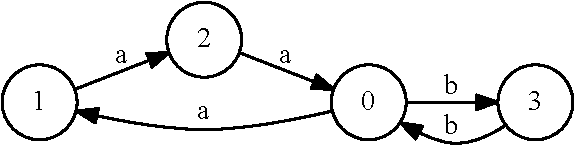
\includegraphics[width=5cm]{pictures/example_graph.pdf}
%  	\]
%  	\pause
%  	\[
%  	\begin{array}{rcclcrccl}
%  	0: & S & \rightarrow & A \ B   & \quad & 3: & A & \rightarrow & \text{\emph{a}}     \\
%  	1: & S & \rightarrow & A \ S_1       & \quad & 4: & B & \rightarrow & \text{\emph{b}} \\
%  	2: & S_1 & \rightarrow & S \ B & & & & &
%  	
%  	\end{array}
%  	\]
%  	
%\end{frame}

%\begin{frame}[fragile] \frametitle{Example: Initial Matrices}
%\[
%T^{(1),A} = \begin{pmatrix}
%\bot & (0,1,0,1,1)       & \bot & \bot       \\
%\bot & \bot & (1,2,1,1,1)       & \bot \\
%(2,0,2,1,1)       & \bot & \bot & \bot \\
%\bot       & \bot & \bot & \bot \\
%\end{pmatrix}
%\]
%\[
%T^{(1),B} = \begin{pmatrix}
%\bot & \bot       & \bot & (0,3,0,1,1)       \\
%\bot & \bot & \bot       & \bot \\
%\bot       & \bot & \bot & \bot \\
%(3,0,3,1,1)      & \bot & \bot & \bot \\
%\end{pmatrix}
%\]
%
%\end{frame}

%\begin{frame}[fragile] \frametitle{Example: Final Matrix}
%\[
%T^{(14),S} = \begin{pmatrix}
%(0,0,1,12,12) & \bot       & \bot & (0,3,1,6,6)       \\
%(1,0,2,4,4) & \bot & \bot       & (1,3,2,10,10) \\
%(2,0,0,8,8)       & \bot & \bot & (2,3,0,2,2) \\
%\bot       & \bot & \bot & \bot \\
%\end{pmatrix}
%\]
%
%\end{frame}

%\begin{frame}[fragile] \frametitle{Path Extraction Algorithm}
%\begin{algorithm}[H]
%	\begin{algorithmic}[1]
%		\caption{Path extraction algorithm}
%		\label{lst:algo3}
%		\Function{extractPath}{$i, j, A, T=\{T^{A_i}\}, G=(N,\Sigma,P)$}
%		\State{$index \gets T^{A}_{i,j}$ }
%		
%		\If{$index = \bot$}
%		\State \Return $\pi_{\emptyset}$
%		\Comment{Such a path does not exist}
%		\EndIf
%		
%		\If{$index.height = 1$}
%		\If{$index.length = 0$}
%		\State \Return $[]$
%		\Comment{Return an empty path}
%		\EndIf
%		\ForAll{$ x \mid (i,x,j) \in E$}
%		\If{$A \to x \in P$}
%		\State \Return $[(i,x,j)]$
%		\Comment{Return a path of length one}
%		\EndIf
%		\EndFor
%		\EndIf
%		
%		\ForAll{$A \to B C \in P$}
%		\State{$index_B \gets T^{B}_{i,index.middle}$ }
%		\State{$index_C \gets T^{C}_{index.middle,j}$ }			
%		\If{$(index_B \neq \bot) \wedge (index_C \neq \bot)$}
%		\State{$maxH \gets max(index_B.height, index_C.height)$ }
%		\If{$index.height = maxH + 1$}
%		
%		
%		\State{$\pi_1 \gets$ \Call{extractPath}{$i, index.middle, B, T, G$}}
%		\State{$\pi_2 \gets$ \Call{extractPath}{$index.middle, j, C, T, G$}}
%		\State \Return $\pi_1 + \pi_2$
%		\Comment{Return the concatenation of paths}
%		\EndIf
%		\EndIf
%		\EndFor
%		\EndFunction
%	\end{algorithmic}
%\end{algorithm}
%\end{frame}


\begin{frame}[fragile] \frametitle{Path extraction}

\begin{itemize}
	\item After constructing a set of matrices with PathIndexes, we can extract the
	required path $i\pi j$ for every node pair $i, j$ and non-terminal $A$ if such path exists
	\pause
	\begin{itemize}
		\item The path which forms a string with minimal height of derivation tree
		\pause
		\item The shortest path
	\end{itemize}
    \pause
	\item Linear complexity in the length of the extracted path
\end{itemize}
\end{frame}


\begin{frame}[fragile] \frametitle{Implementations}

\begin{itemize}
	\item We use \textbf{RedisGraph} graph database as storage
	\pause
	\item \textbf{CPU-based} implementations use \textbf{SuiteSparse} implementation
	of \textbf{GraphBLAS}, which provides a set of sparse matrix operations
	\begin{itemize}
		\item $\textbf{RG\_CPU}_{\textit{rel}}$ --- for the relation query semantics
		\pause
		\item $\textbf{RG\_CPU}_{\textit{path}}$ --- for the single-path query semantics
	\end{itemize}
	\pause
	\item \textbf{GPGPU-based} implementations with sparse matrix representation
	\begin{itemize}
		\item $\textbf{RG\_CUSP}_{\textit{rel}}$ --- relational query semantics, utilizes a \textbf{CUSP} library for matrix operations
		\pause
		\item $\textbf{RG\_SPARSE}_{\textit{rel}}$ --- relational query semantics, uses low-latency on-chip shared memory for the hash table of each row of the result matrix
		\pause
		\item $\textbf{RG\_SPARSE}_{\textit{path}}$ --- single-path query semantics, operating over PathIndex semiring
	\end{itemize}
\end{itemize}
\end{frame}


\begin{frame}[fragile] \frametitle{Dataset\footnote{Queries is based on the context-free grammars for 
		nested parentheses}}
\begin{center}
 {\small
	\setlength{\tabcolsep}{0.4em}
	\rowcolors{2}{}{lightgray}
	\begin{tabular}{| l | c | c |}
		\hline
		RDF Name                  & \#V    & \#E \\
		\hline
		\hline
		univ-bench					& 179		& 413\\
		pizza						& 671		& 2,604\\
		wine							& 733		& 2,450\\
		core							& 1,323		& 8,684\\
		pathways						& 6,238		& 37,196\\
		go-hierarchy					& 45,007		& 1,960,436    \\
		enzyme						& 48,815		& 219,390     \\
		eclass\_514en				& 239,111		& 1,047,454        \\
		go							& 272,770		& 1,068,622    \\
		geospecies							& 450,609		& 4,622,922    \\
		\hline
	\end{tabular}
}
\end{center} 
\end{frame}

\begin{frame} \frametitle{Evaluation}
  \begin{itemize}
   \item OS: Ubuntu 18.04
   \item CPU: Intel core i7 6700 3,4GHz
   \item RAM: DDR4 64 Gb
   \item GPGPU: NVIDIA GeForce 1070 (8Gb RAM)
  \end{itemize}
\end{frame}

\begin{frame}[fragile] \frametitle{Evaluation: CFPQ\footnote{Time in seconds and memory is measured in megabytes}}
\begin{center}
	\tikzmark{yyy}{
	}
	{\tiny
	{\setlength{\tabcolsep}{0.4em}
			\rowcolors{3}{}{lightgray}
			\begin{tabular}{| l | r  r | r  r | r  r | r  r | r  r |}
				\hline
				
				\multirow{3}{*}{Name}   &   \multicolumn{6}{|c|}{Relational semantics index}	&	\multicolumn{4}{|c|}{Single path semantics index} \\
				\cline{2-11}
				&	\multicolumn{2}{|c|}{RG\_CPU\textsubscript{rel}}	&	\multicolumn{2}{|c|}{RG\_CUSP\textsubscript{rel}}	&	\multicolumn{2}{|c|}{RG\_SPARSE\textsubscript{rel}} &	\multicolumn{2}{|c|}{RG\_CPU\textsubscript{path}}	&	\multicolumn{2}{|c|}{RG\_SPARSE\textsubscript{path}}	 \\
				\cline{2-11}
				&   Time & Mem &  Time     & Mem & Time     & Mem  &  Time     & Mem & Time     & Mem \\
				\hline
				\hline
				core                        & 0.004 & 0.3  & 0.022 & 2.0   & 0.010  & 0.1      & 0.002 & 0.3  & 0.016 & 0.1  \\
				eclass\_514en                 & 0.067 & 13.8 & 0.075 & 14.0  & 0.166 & 16.0     & 0.195 & 31.2 & 0.496 & 26.0   \\
				enzyme                      & 0.018 & 5.9  & 0.021 & 0.1 & 0.018 & 4.0        & 0.029 & 8.1  & 0.043 & 6.0    \\
				go-hierarchy                & 0.091 & 16.3 & 0.433 & 650.0 & 0.108 & 121.2    & 0.976 & 92.0   & 0.336 & 125.0  \\
				go                          & 0.604 & 28.8 & 0.590  & 70.0  & 0.365 & 30.2     & 1.286 & 75.7 & 0.739 & 45.4 \\
				pathways                    & 0.011 & 0.1  & 0.019 & 0.1 & 0.007 & 0.1      & 0.021 & 0.5  & 0.021 & 2.0    \\	
				univ-bench                  & 0.002 & 0.3  & 0.010  & 0.1 & 0.005 & 0.1      & 0.013 & 0.3  & 0.007 & 0.1  \\
				pizza                       & 0.030  & 1.8  & 0.021 & 4.0   & 0.006 & 0.1      & 0.075 & 5.5  & 0.009 & 0.1  \\
				wine                        & 0.017 & 3.5  & 0.032 & 6.0   & 0.009 & 0.1      & 0.117 & 7.1  & 0.015 & 0.2  \\
				geospecies & 7.146 & 16934.2 & --- & --- & 0.856 & 5274 & 15.134 & 35803.6 & 1.935 & 5282   \\
				\hline
			\end{tabular}
	}
}
 \end{center}
%\pause
%\onslide<2>{\tikz[overlay,remember picture]{\draw[draw=red,thick,fill opacity=0.2] ($ (yyy) + (5.5,0.01)$) rectangle ($ (yyy) + (8.1,-4.5)$);}}

\end{frame}

\begin{frame}[fragile] \frametitle{Evaluation: Path Extraction Time For \textit{go}}
\begin{center}
    \[
		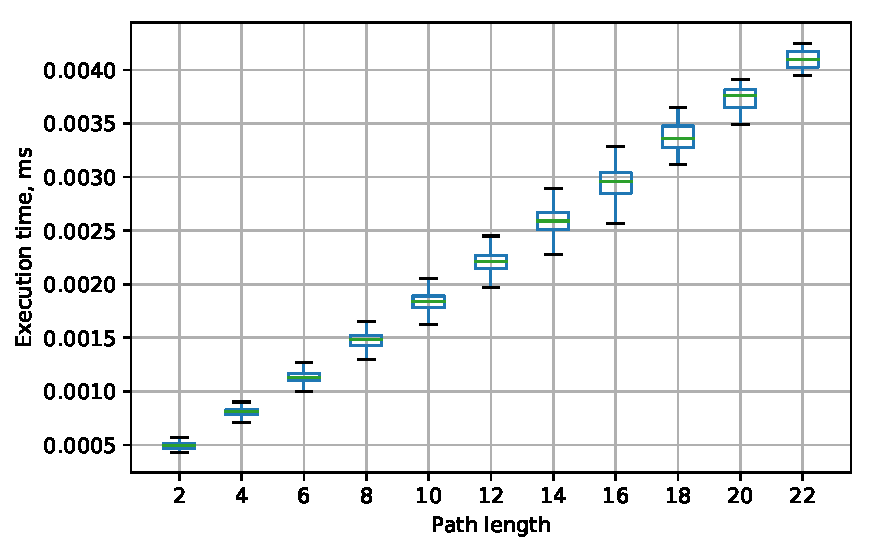
\includegraphics[width=\linewidth,trim=0 0 -1.5cm 0]{plots/G1_go.pdf}
	\]
\end{center}

\end{frame}

\begin{frame}[fragile] \frametitle{Evaluation: Path Extraction Time For \textit{geospecies}}
\begin{center}
	\[
	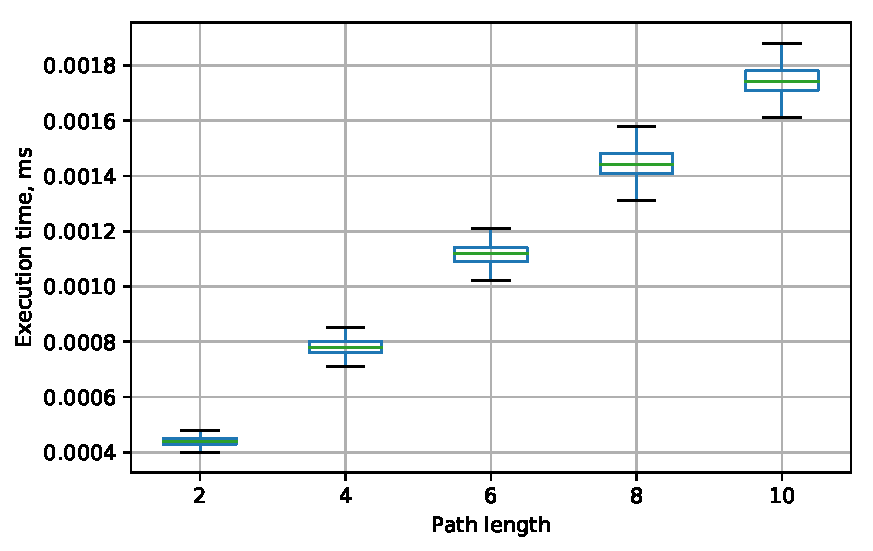
\includegraphics[width=\linewidth,trim=0 0 -1.5cm 0]{plots/Geo_geospicies.pdf}
	\]
\end{center}

\end{frame}

\begin{frame}[fragile] \frametitle{Conclusion}
  \begin{itemize}
    \item GPGPUs utilization significantly increases the performance of CFPQ for both query semantics
    \pause
    \item Implementations with sparse matrix representation are significantly faster than others
    \pause
    \item The cost of computing matrices with PathIndexes for single-path query semantics is not high
    \pause
    \item The additional running time of the path extraction is small and linear in the length of the path
    \pause 
    \item The matrix-based algorithm paired with a suitable database is a promising way to make CFPQ applicable for
    real-world data analysis
  \end{itemize}
  \pause
  \begin{itemize}
    \item Dataset is published: both graphs and queries
    \begin{itemize}
    	\item Link: \url{https://github.com/JetBrains-Research/CFPQ_Data}
    \end{itemize}
    
    \item Implementations are available on GitHub
    \begin{itemize}
    	\item Link: \url{https://github.com/YaccConstructor/RedisGraph}
    \end{itemize}
    
  \end{itemize}
\end{frame}

\begin{frame}[fragile] \frametitle{Future Research}
  \begin{itemize}
  	\item Extend the matrix-based CFPQ algorithm to all-path
  	query semantics
  	\pause
  	\item Update the query results dynamically when data changes
  	\pause
    \item Improve the dataset
    \begin{itemize}
      \item Include real-world cases from
      the area of static code analysis
      \item Find new applications that required CFPQ, such as graph
      segmentation
    \end{itemize}
\end{itemize}
\end{frame}

\begin{frame}
\frametitle{Acknowledgments}
\begin{itemize}
	\item Special thanks to
	\begin{itemize}
		\item Gábor Szárnyas for informing about SuiteSparse on the previous GRADES
		\item George Fletcher for informing about the measurements with the graph databases on the previous GRADES
		\item Roi Lipman for great help with RedisGraph graph database
	\end{itemize}
\end{itemize}
\end{frame}

\begin{frame}
\frametitle{Contact Information}
\begin{itemize}
  \item Semyon Grigorev:
    \begin{itemize}
      \item \href{mailto:s.v.grigoriev@spbu.ru}{s.v.grigoriev@spbu.ru}
      \item \href{mailto:Semen.Grigorev@jetbrains.com}{Semen.Grigorev@jetbrains.com}
    \end{itemize}
  \item Rustam Azimov:
  \begin{itemize}
  	\item \href{mailto:rustam.azimov19021995@gmail.com}{rustam.azimov19021995@gmail.com}
  	\item \href{mailto:Rustam.Azimov@jetbrains.com}{Rustam.Azimov@jetbrains.com}
  \end{itemize}
  \item Arseniy Terekhov: \href{mailto:simpletondl@yandex.ru}{simpletondl@yandex.ru}
  \item Artyom Khoroshev: \href{mailto:arthoroshev@gmail.com}{arthoroshev@gmail.com}
\vspace{0.5cm}
  \item Dataset: \href{https://github.com/JetBrains-Research/CFPQ_Data}{https://github.com/JetBrains-Research/CFPQ\_Data}
   \item Algorithm implementations: \href{https://github.com/YaccConstructor/RedisGraph}{https://github.com/YaccConstructor/RedisGraph}
\end{itemize}
\vspace{0.1cm}
\center{\huge{Thanks!}}
\end{frame}
\end{document}
